\chapter{Projektbeschreibung}
\label{ch:description}
Der Titel des Projekts lautet \enquote{Automatische DNS-Zonen und Eintragsverwaltung in einer verteilten Multi-Cloud-Microservice-Architektur} und wird im Folgenden beschrieben.
Diese Arbeit soll sich auf das Kernthema der automatischen DNS-Zonen und Eintragsverwaltung in einer verteilten Multi-Cloud-Microservice-Architektur konzentrieren und nicht auf die Implementierung der Microservices selbst.
\ac{DNS} bietet Namensauflösung für das Internet, indem es menschenlesbare Namen (z. B. example.com) in maschinenroutenfähige IP-Adressen (unter anderem) umwandelt. ~\cite{chung2017understanding}.
Weiterhin werden verwendete Technologien welche nicht direkt mit dem Kernthema in Verbindung stehen nur oberflächlich behandelt.

\section{Idee}
\label{sec:description:projektidee}
Die Projektidee entstand aus dem Bedarf der Prozesstrennung und Automatisierung zwischen den Abteilungen der Entwicklung und dem Betrieb.

\subsection{Ziel}
\label{subsec:description:ziel}
Die Abteilung des Betriebs besteht aus \ac{DevOps}, welche sich um die Entwicklung und Bereitstellung von Infrastruktur kümmert.
Die Abteilungen der Entwickler beschäftigen sich mit der Entwicklung von Microservices und der Bereitstellung dieser auf der Infrastruktur.
Microservices bezeichnen einen Ausbau einer Programm-Architektur, bei der ein Programm in mehrere kleine Programme aufgeteilt wird, welche jeweils eine Aufgabe erfüllen und mit anderen Teilen des Programms über \ac{API}s kommunizieren ~\cite{redhead-kubernetes:2023}.
So ist ein Microservice eine kleine, unabhängige Komponente, welche eine Aufgabe erfüllt und mit anderen Microservices kommuniziert.
Ein logischer Zusammenschluss aus mehreren Microservices bildet eine Anwendung, auch \enquote{service} genannt.
\medskip

Diese Infrastruktur wird auf Kundenwünsch hin auf verschiedenen Cloud-Providern bereitgestellt.
Das Ziel der Arbeit ist den Entwicklern die Bereitstellung ihrer Microservices auf verschiedenen Cloud-Providern zu ermöglichen, ohne dass sie sich mit den Cloud-Providern beschäftigen müssen
und ihnen eine adequate Abstraktionsebene zu bieten, welche die Komplexität der Cloud-Provider verbirgt und Prozesse außerhalb dieser Ebene automatisiert.
\medskip

Fokus der Arbeit ist hierbei die automatisierung von \ac{DNS}.
DNS ist ein System, welches Domainnamen in IP-Adressen auflöst und somit die Erreichbarkeit ermöglicht um Oberflächen oder APIs aufrufen zu können ~\cite{klensin2003role}.
\medskip

Weiterhin müssen alle Ergebnisse dieser Arbeit dem neuesten Stand der Technik entsprechen und die Sicherheit der Infrastruktur gewährleisten.
So wurden vorab die Anforderungen an Private Zonen und DNSSEC ermittelt, welche im Verlauf der Arbeit genauer beschrieben werden.
Private Zonen sind Zonen, welche nur innerhalb des Netzwerks erreichbar sind und somit die Sicherheit erhöhen, da IP-Adressen nicht öffentlich sichtbar sind.
DNSSEC ist eine Erweiterung von DNS, welche die Authentizität und Integrität von DNS-Einträgen gewährleistet und somit die Sicherheit erhöht ~\cite{arends2005rfc}.

\subsection{Motivation}
\label{subsec:description:motivation}
Für die Wahl der Abstraktionsebene gibt es viele Faktoren, welche nicht in gänze in dieser Arbeit behandelt werden können.
Die Wahl fiel auf Kubernetes, da es sich um eine Open-Source Software handelt, welche Funktionen und Interfaces zur Verfügung stellt, um Microservices zu entwickeln und bereitzustellen.
Kubernetes ist, nach Stand der Dinge, der Standard für Container Orchestration ~\cite[p.~2]{SpringerNature:2022}.
Auf Kubernetes wird im Abschnitt \ref{subsec:description:umfeld} genauer eingegangen.
\medskip
Damit ein auf Kubernetes bereitgestellter Microservice von außerhalb des Kubernetes Clusters (z.B. aus dem Internet) erreichbar ist, muss ein \ac{DNS}-Eintrag erstellt werden.
Das sich nun stellende Problem besteht darin, dass die Microservices auf Kubernetes bereitgestellt werden, jedoch DNS-Einträge, welche für die Erreichbarkeit des Microservices sorgen, teil des Cloud-Providers sind und außerhalb von Kubernetes verwaltet werden.
Dadurch entstand eine manuelle Tätigkeit, welche die Entwickler von ihrer eigentlichen Arbeit und Aufgabenbereich abhält und somit die Effizienz der Entwickler verringert.
Schlussfolgernd ist für die SDA SE wünschenswert, den Zugriff der Entwickler so weit wie möglich auf lediglich Kubernetes zu beschränken und direkten Zugriff auf die Cloud-Provider zu vermeiden.
\medskip

So entstand die Motivation, DNS-Einträge automatisch anhand der in Kubernetes enthaltenen Informationen zu erstellen und zu verwalten.

\section{Planung}
\label{sec:description:planung}
Bei der Planung muss zwingend auf die Skalierbarkeit und Erweiterbarkeit der Lösung geachtet werden, da die SDA SE ein stark wachsendes Unternehmen ist und die Lösung auch in Zukunft noch verwendet werden soll.
Außerdem muss die Lösung so gestaltet werden, dass sie auf verschiedenen Cloud-Providern funktioniert, da die SDA SE Microservices auf verschiedenen Cloud-Providern bereitstellt.
Weiterhin ist das Lizenzmodell von verwendeten Lösungen zu beachten, da die SDA SE eine Open-Source first Policy verfolgt und somit Open-Source Lösungen bevorzugt werden.

\subsection{Umfeld}
\label{subsec:description:umfeld}
Die Laufzeitumgebung der Microservices ist Kubernetes, welches auf den Cloud-Providern \ac{AWS}, \ac{GCP} und \ac{Azure} als verwalteter Service gebucht wird.
Kubernetes ist ein Container-Orchestrierungssystem, welches die Bereitstellung, Skalierung und Verwaltung von Containern ermöglicht.
Die Microservices werden in den Programmiersprachen Java, Python und Golang entwickelt und in Docker Container-Images verpackt, was die enthaltenen Programmzeilen, Bibliotheken und Abhängigkeiten kapselt und somit eine effiziente Bereitstellung, Skalierung, Unveränderbarkeit und Verbreitung auf Kubernetes ermöglicht ~\cite{rad2017introduction}.
Ein Docker Container-Image ist eine Datei, welche alle Abhängigkeiten und Konfigurationen enthält, um ein Programm zu starten und ist prinzipiell einer virtuellen Maschine sehr ähnlich nur, dass der Kernel des Hosts mitverwendet wird ~\cite[p.~229]{rad2017introduction}.
\medskip

Die implementierung mehrerer Cloud-Provider ist notwendig, da die Microservices aufgrund von Kundenanforderungen auf verschiedenen Cloud-Providern bereitgestellt werden müssen.
Ein Kunde kann beispielsweise die Bereitstellung seiner Microservices auf AWS fordern, während ein anderer Kunde die Bereitstellung auf GCP oder Azure fordert.
Die Wahl des Cloud-Providers ist für Kunden eine essenzielle Entscheidung, da Kunden komplexe Verträge mit den Cloud-Providern abschließen und diese nicht ohne weiteres wechseln können.
\medskip

Das Bereitstellen von Kubernetes auf verschiedenen Cloud-Providern ist eine komplexe Aufgabe, da die Cloud-Provider gänzlich unterschiedliche Herangehensweisen und Anforderungen haben.
Der Aufbau der Infrastruktur auf AWS unterscheidet sich grundlegend von dem Aufbau auf GCP oder Azure, was einer vollständigen Automatisierung nicht gerade in die Hände spielt ~\cite[p.~450]{khot2020comparative}.
Neue Initiativen wie \ac{CAPI} versuchen diese Problematik zu lösen, benötigen jedoch auch viel Provider-spezifischen Code, was die Komplexität dadurch nicht verringert.
Außerdem wird für diesen Ansatz ein management Kubernetes Cluster benötigt, welcher sich nicht selbst bootstrappen kann und somit zumindest initial ein anderer Ansatz gewählt werden muss.
Bei der SDA SE wurde sich für eine \ac{IaC} Herangehensweise entschieden, welche die Infrastruktur auf den Cloud-Providern mittels Terraform bereitstellt.
IaC ist ein Ansatz, bei dem die Infrastruktur mittels Code deklarativ beschrieben wird und somit eine automatisierte Bereitstellung ermöglicht.
Terraform ist ein Open-Source Tool, welches die Infrastruktur auf verschiedenen Cloud-Providern bereitstellen kann, wohingegen ein konkurrierendes Tool wie CloudFormation nur mit AWS funktioniert.
\medskip

Trotz der Unterschiede bei den Cloud-Providern einen Kubernetes Cluster zu provisionieren, sind die Kubernetes Cluster implementationen bei den Cloud-Providern selbst beinahe identisch.
Diesen Umstand will sich die SDA SE zunutze machen und Kubernetes als Abstraktionsebene zwischen den Cloud-Providern und weiterer Infrastruktur nutzen, um die Komplexität vor den Entwicklern zu verbergen.
Die Entwickler sollen sich nicht mit allen Feinheiten der Infrastruktur beschäftigen müssen, sondern lediglich Kubernetes nutzen, um ihre Microservices zu entwickeln und bereitzustellen, um ihre Arbeitszeit effizienter nutzen zu können.
Um dies zu erreichen und die Entwickler so gut wie möglich mit automatischen Produktionsstrassen zu unterstützen, kann Kubernetes in seiner Funktion mit weiteren Programmen (auch Operatoren genannt) erweitert und ausgebaut werden.
Ein solcher Ausbau wird häufig als Plattform bezeichnet.
\medskip

So ist das Produkt der SDA SE eine Plattform (genannt \enquote{nimbusKube}), welche die Bereitstellung von Microservices auf verschiedenen Cloud-Providern mittels Kubernetes ermöglicht und erleichtert.
Eine simultane Bereitstellung auf mehreren Cloud-Providern gleichzeitig ist möglich, jedoch im Standard nicht vorgesehen.

Eine Bestellung dieser Plattform enthält bis zu vier Kubernetes Clustern, welche auf dem gewählten Cloud-Provider bereitgestellt werden.
Die Anzahl der Cluster ist abhängig von der Anzahl der gewünschten Umgebungen.
So ist die kleinste Bestellung eine Umgebung mit zwei Clustern, einem \enquote{Tools} und einem \enquote{Development} Cluster.
Der Tools Cluster ist für die Bereitstellung von Plattform-Tools zuständig, welche für die Entwicklung und Bereitstellung von Microservices benötigt werden.
Die Umgebungscluster \enquote{Development}, \enquote{Staging} und \enquote{Production} sind einzig zuständig für das Bereitstellen von Firmen-Logik spezifischer Software.

\subsection{Plan}
\label{subsec:description:plan}

Zur Projektplanung wurde ein iteratives Vorgehensmodell gewählt, da die Anforderungen und Auswirkungen des Projekts nicht vollständig bekannt sind und sich im Laufe des Projekts ändern können.
Es wird außerdem angenommen, dass eine Konzeption sich später beim Test als unbefriedigend herausstellen könnte und somit ein Zurückkehren zur Konzeptionsphase notwendig sein könnte.

\begin{table}[H]
  \begin{tabular}{ |p{3cm}|p{6cm}|p{3cm}| }
      \hline
      \textbf{Phase}                    &      \textbf{Tätigkeiten}                 &    \textbf{Dauer (Stunden)} \\
      \hline
      \hline
      Anforderungen                     &      Ziel definieren                      &    3               \\
      \hline
      \multirow{3}{*}{Analyse}          &      Vergleich Kubernetes Operatoren      &    5               \\
                                        &      Funktionsweise DNSSEC                &    5               \\
                                        &      Funktionsweise Public/Private        &    3               \\
      \hline
      \multirow{4}{*}{Konzeption}       &      DNS Hierarchie                       &    5               \\
                                        &      Security Öffentlich/Private Zonen    &    5               \\
                                        &      Security DNSSEC                      &    5               \\
                                        &      Infrastruktur Übersetzung            &    2               \\
      \hline
      \multirow{5}{*}{Implementierung}  &      DNS Hierarchie                       &    10              \\
                                        &      Security Öffentlich/Private Zonen    &    15              \\
                                        &      Security DNSSEC                      &    10              \\
                                        &      Infrastruktur Übersetzung            &    5               \\
                                        &      Kubernetes Operator                  &    10              \\
      \hline
      Test                              &      Testen der Erstellung                &    10              \\
                                        &      Testen der Erreichbarkeit            &    3               \\
      \hline
      Übergabe                          &      Übergabe per IaC                     &    0               \\
      \hline
      \hline
      \textbf{Gesamt}                   &                                           &    100             \\
      \hline
  \end{tabular}
  \caption[Projektplan]{Projektplan}
  \label{subsec:description:plan:table}
\end{table}

\subsection{Wirtschaftlichkeitsbetrachtung}
\label{subsec:description:wirtschaftlichkeitsbetrachtung}
Da zusätzliche Infrastrukturkosten derart gering sind, dass sie vernachlässigt werden können, wird sich die Wirtschaftlichkeitsbetrachtung auf die Arbeitszeit beschränken.
So ist beispielhaft das Kostenmodell für DNS auf AWS nach Aufrufen gestaffelt und diese sind unabhängig vom Projekt gleich.
Weiterhin sind die Kosten von Servern im Kubernetes auch unabhängig vom Projekt gleich, da ein Operator sehr geringe Lastkosten verursacht.

Die Projektlaufzeit wurde nach ~\ref{subsec:description:plan:table} auf 100 Stunden geschätzt.
Die anfallende Arbeitszeit für die manuelle Erstellung DNS Einträge wurde auf 5 Minuten pro Eintrag geschätzt.
Bei ungefähr 300 ausgerollten Microservices pro Tag (aus GitHub der SDA SE ausgelesen), ist der Break-Even-Point nach 4 Tagen erreicht.

\subsection{Alternativen}
\label{subsec:description:alternativen}
Als alternative für den Ansatz welcher bereits in Teilen in dieser Arbeit präsentiert wurde, gibt es die Möglichkeit Wildcard DNS Einträge zu verwenden.
Diese Einträge sind Platzhalter für alle Subdomains einer Domain und können auch zur Auflösung verwendet werden.
Dieser Vorgang wäre nicht auf die Erstellung einzelner Einträge angewiesen, sondern würde alle Subdomains einer Domain auflösen.
\medskip

Dieser Ansatz erschwert jedoch die gewünschte Trennung in öffentliche und private Zonen, da sonst eine Subdomain zur Unterscheidung zwischen öffentlich und privat verwendet werden müsste.
Auf die gewünschte Struktur der Zonen und Begründungen dieser wird im Abschnitt ~\ref{sec:description:umsetzung} genauer eingegangen.

\section{Umsetzung}
\label{sec:description:umsetzung}
Diese Sektion befasst sich dem Verlauf der Realisierung des Projekts, der Organisation und den dabei aufgetretenen Problemen.

\subsection{Organisation}
\label{subsec:description:Organisation}
Diese Arbeit wurde eigenständig und ohne direkte Anleitung durchgeführt.
Die Organisation der Arbeit und der Arbeitsergebnisse wurde durch wöchentliche Meetings mit dem Auftraggeber sichergestellt.

Analysen und Konzepte wurden in Form von Dokumenten festgehalten und dem Auftraggeber zur Verfügung gestellt.
Die Implementierung wurde in Form von Code in einem GitHub Repository festgehalten und dem Auftraggeber zur Verfügung gestellt.

\subsection{Verlauf}
\label{subsec:description:verlauf}
Es wurde ein iteratives Modell gewählt, welche die Phasen Anforderungen, Analyse, Konzeption, Implementierung, Test immer wieder durchläuft.
Eine Anforderung wurde definiert, der Ist-Zustand analysiert, ein Konzept erstellt um sich der Anforderung so weit wie möglich anzunähern, dieses Konzept implementiert und getestet.
Daraufhin wurde die Anforderung erneut betrachtet und gegebenenfalls angepasst.
Beim zufriedenstellenden Ergebnis wurde die nächste Anforderung betrachtet und der Prozess wiederholt.
Mit dem Abschließen der letzten Anforderung, wurden die Ergebnisse in ihrer Gänze betrachtet, getestet und gegebenenfalls angepasst.
Am Ende der Arbeit wurde die Übergabe der Ergebnisse an den Auftraggeber durchgeführt.

\section{Ergebnisse}
\label{sec:description:ergebnisse}
Diese Sektion befasst sich mit den Ergebnissen der Arbeit und der Wirtschaftlichkeitsbetrachtung.

\subsection{Darstellung}
\label{subsec:description:darstellung}
Das erste zu präsentierende Ergebnis ist die Auswahl des Kubernetes Operators.
Hierbei wurde sich für den Operator \enquote{external-dns} entschieden, da dieser die gewünschten Funktionen bietet und die SDA SE bereits Erfahrung mit diesem Operator hat.
Dieser Operator ist aktuell der einzige Open-Source Operator, welcher die gewünschten Funktionen bietet.
\medskip

Als nächstes soll die DNS Hierarchie dargestellt werden.
Die Domain ist \enquote{sda-se.io}, wobei die \ac{TLD} (io) bei einem externen Registrar registriert ist.
Registrare sind Organisationen, die Domainnamen verkaufen und häufig die autoritativen Nameserver betreiben ~\cite{chung2017understanding}.

In einem AWS Konto, beispielsweise mit dem Namen \enquote{DNS-Root}, werden nun eine private (private) und eine öffentliche (public) Zone für \enquote{sda-se.io} erstellt.
Die Nameserver der öffentlichen Domain werden beim Registrar eingetragen, um zur öffentlichen Zone zu delegieren.
\medskip

Wird eine Bestellung der Plattform getätigt, werden in einem beliebigen Cloud-Provider (z.B. AWS) weitere Zonen erstellt.
Die Bestellung der Plattform erhält einen Projektnamen, welcher als Subdomain der Domain verwendet wird, zum Beispiel \enquote{projekt1}.
Für diesen Namen werden in dem Zielkonto eine öffentliche und eine private Zone erstellt und die private Zone mit dem \ac{VPC} der Plattform assoziiert.
Mit einem AWS VPC kann eine logisch isolierte Sektion der AWS-Cloud bereitgestellt werden, in der AWS-Ressourcen in einem definierten virtuellen Netzwerk gestartet werden können ~\cite[p.~12]{mathew2014overview}.
Über diese Assoziation wird implizit \enquote{DNS Split-Horizon} konfiguriert.
Split-horizon DNS, auch als Split-View DNS, Split-Brain DNS oder Split DNS bekannt, ermöglicht es, verschiedene Sätze von DNS-Informationen bereitzustellen, die
in der Regel durch die Quelladresse der DNS-Anfrage ausgewählt werden.
Diese Funktion bietet einen Mechanismus für das Management von Sicherheit und Privatsphäre durch die logische oder
physische Trennung von DNS-Informationen für den Netzwerk internen Zugriff ~\cite{wikipedia:split-horizon}.
\medskip

Weiterhin wird für jede Umgebung, die dazu bestellt wurde, ein weiterer Satz Zonen erstellt (privat und öffentlich), welche die Subdomain der Umgebung enthält (außer Produktion, diese Umgebung verwendet die Projekt-Subdomain).
So werden für die Umgebung \enquote{Development} die Zonen für \enquote{dev.projekt1.sda-se.io} erstellt.
\medskip

Für die Veröffentlichung eines Services wird eine \enquote{VirtualService} Resource in Kubernetes erstellt, welches die gewünschte Subdomain enthält.
Ein VirtualService ist eine Kubernetes Resource, welche von dem Istio Service Mesh verwendet wird, um die Veröffentlichung von Services zu ermöglichen.
Istio ist ein Service-Mesh, dass die Netzwerkkommunikation zwischen Mikrodiensten in einer Kubernetes-Umgebung verwaltet, überwacht und sichert.
\medskip

In dem VirtualService wird die gewünschte Subdomain des Services angegeben, welche vom Operator \enquote{external-dns} beobachtet werden muss.
Außerdem muss ein Istio Ingress Gateway angegeben werden (privat oder öffentlich).
Der Operator \enquote{external-dns} beobachtet die VirtualService Resource und erstellt automatisch einen DNS-Eintrag in der entsprechenden Zone.
\medskip

Nachdem ein grundlegendes Verständnis für diesen Prozess geschaffen wurde, kann nun die Sicherheit der Zonen betrachtet werden.
Öffentliche Zonen sollten nur DNS-Einträge öffentlicher Services enthalten, bei denen die veröffentlichung der Einträge unabdingbar ist.
DNS-Einträge privater Services sollten nur in privaten Zonen enthalten sein, welche nur innerhalb des Netzwerks erreichbar sind, damit eventuelle Angreifer
keine Informationen über die Infrastruktur erhalten können.
Dies wird mittels Split-Horizon DNS und der Konfiguration von external-dns erreicht.
Jede Zone erhält eine Installation des Operators external-dns.
Die Installation der öffentlichen Zone erstellt nur die DNS-Einträge der öffentlichen Services in der öffentlichen Zone.
Die Installation der privaten Zone erstellt alle DNS-Einträge, jene der privaten als auch die der öffentlichen Services in der privaten Zone.
Anfragen, welche aus dem Internet erfolgen, werden an die öffentliche Zone delegiert und erhalten nur die DNS-Einträge der öffentlichen Services.
Anfragen, welche aus dem privaten Netzwerk erfolgen, werden an die private Zone delegiert (Split-Horizon) und erhalten alle DNS-Einträge, jene der privaten als auch die der öffentlichen Services.
\medskip

\begin{figure}[htbp]
    \centering
    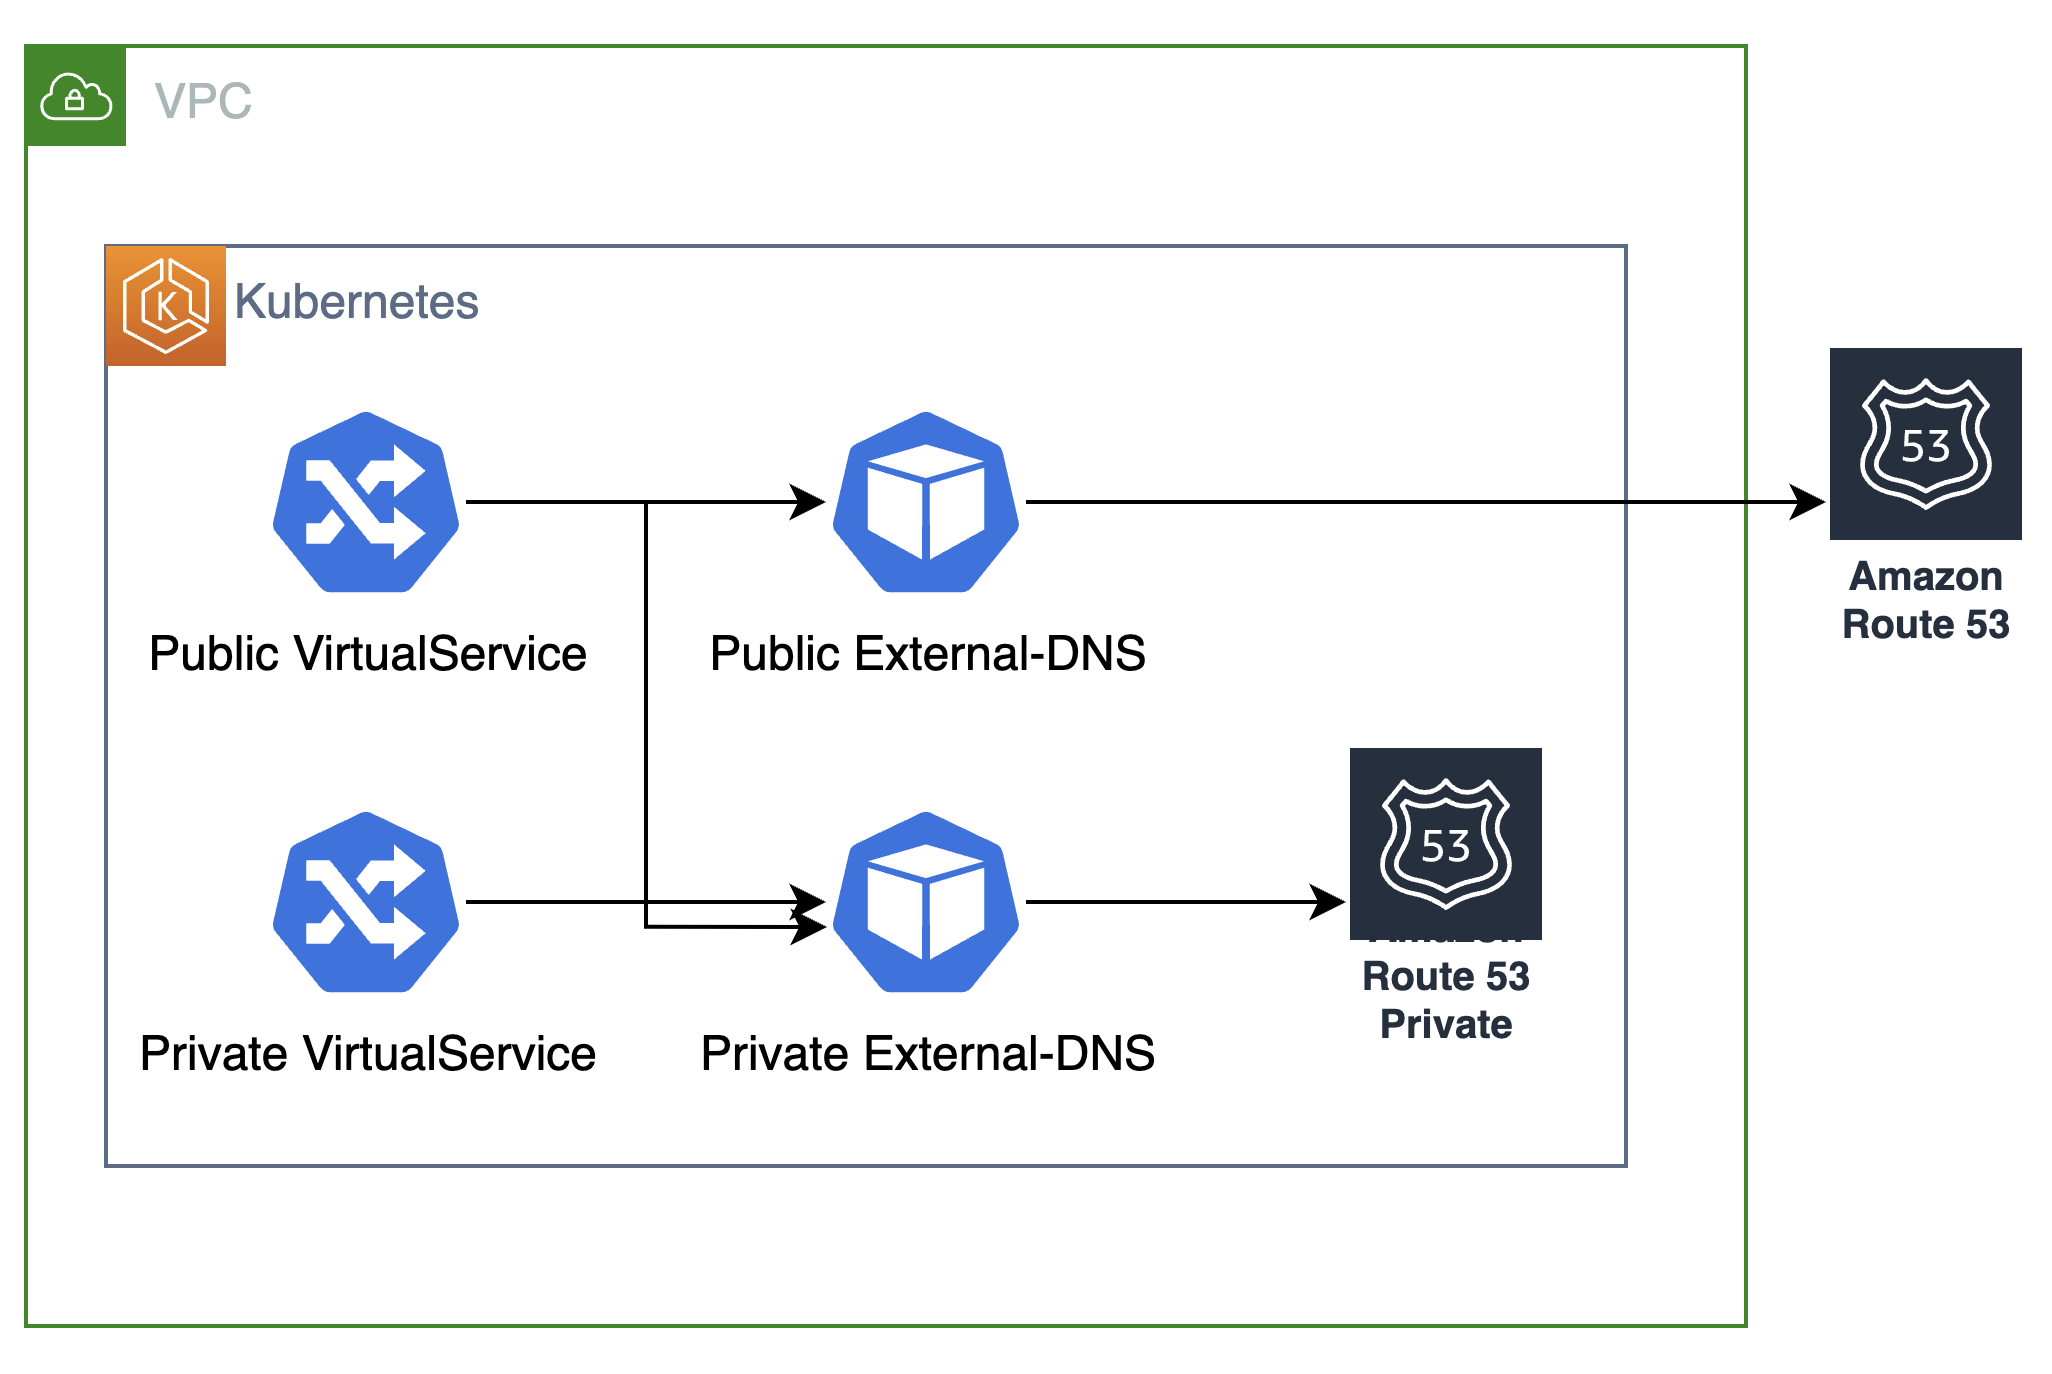
\includegraphics[width=0.9\textwidth]{gfx/now-external-dns}
    \caption{Private und öffentliche Zonenverwaltung mit external-dns}
    \label{fig:Projektbeschreibung:external-dns}
\end{figure}

Ein in Kubernetes veröffentlichter Service, zum Beispiel \enquote{service1}, wird in der VirtualService Resource mit der Subdomain \enquote{service1.dev.projekt1.sda-se.io} angegeben und als öffentlicher Service konfiguriert in dem es an das öffentliche Istio Ingress Gateway gebunden wird.
So wird der Service mit seiner Subdomain in sowohl der öffentlichen als auch der privaten Zone erstellt.
\medskip

Die Sicherheit der Zonen wird durch die Verwendung von \ac{DNSSEC} gewährleistet.
DNSSEC ist eine Erweiterung von DNS, welche die Authentizität und Integrität von DNS-Einträgen gewährleistet und somit die Sicherheit erhöht ~\cite{kelm2001sicherheit}.
Um bei AWS DNSSEC zu aktivieren, muss ein KMS-Schlüssel erstellt werden, welcher für die Signierung der DNS-Einträge verwendet wird.
Dieser Schlüssel wird in der Route53 Zone angegeben und aktiviert DNSSEC für diese Zone.
\medskip

\begin{lstlisting}[language=Python,frame=tb,caption={DNSSEC mit Terraform},label={lst:dnssec}]
provider "aws" {
  region = "eu-central-1"
}

data "aws_caller_identity" "current" {}

resource "aws_kms_key" "dnssec_key" {
  customer_master_key_spec = "ECC_NIST_P256"
  deletion_window_in_days  = 7
  key_usage                = "SIGN_VERIFY"
  policy = jsonencode({
    Statement = [
      {
        Action = [
          "kms:DescribeKey",
          "kms:GetPublicKey",
          "kms:Sign",
        ],
        Effect = "Allow",
        Principal = {
          Service = "dnssec-route53.amazonaws.com"
        },
        Sid      = "Allow Route 53 DNSSEC Service",
        Resource = "*",
        Condition = {
          StringEquals = {
            "aws:SourceAccount" = data.aws_caller_identity.current.account_id
          },
          ArnLike = {
            "aws:SourceArn" = "arn:aws:route53:::hostedzone/*"
          }
        }
      },
      {
        Action = "kms:CreateGrant",
        Effect = "Allow",
        Principal = {
          Service = "dnssec-route53.amazonaws.com"
        },
        Sid      = "Allow Route 53 DNSSEC Service to CreateGrant",
        Resource = "*",
        Condition = {
          Bool = {
            "kms:GrantIsForAWSResource" = "true"
          }
        }
      },
      {
        Action = "kms:*",
        Effect = "Allow",
        Principal = {
          AWS = "arn:aws:iam::${data.aws_caller_identity.current.account_id}:root"
        },
        Resource = "*",
        Sid      = "Enable IAM User Permissions"
      },
    ],
    Version = "2012-10-17"
  })
}

resource "aws_route53_zone" "sda_se_io_zone" {
  name = "sda-se.io"
}

resource "aws_route53_zone" "projekt1_sda_se_io_zone" {
  name = "projekt1.sda-se.io"
  delegation_set {
    name_servers = aws_route53_zone.sda_se_io_zone.name_servers
  }
}

resource "aws_route53_zone" "dev_projekt1_public_zone" {
  name = "dev.projekt1.sda-se.io"
  delegation_set {
    name_servers = aws_route53_zone.projekt1_sda_se_io_zone.name_servers
  }
}

resource "aws_route53_zone" "dev_projekt1_private_zone" {
  name              = "dev.projekt1.sda-se.io"
  vpc {
    vpc_id = "your_private_vpc_id"  # Replace with your actual VPC ID
  }
  delegation_set {
    name_servers = aws_route53_zone.projekt1_sda_se_io_zone.name_servers
  }
}

resource "aws_route53_record" "sda_se_io_to_projekt1" {
  zone_id = aws_route53_zone.sda_se_io_zone.zone_id
  name    = "projekt1"
  type    = "NS"
  ttl     = 300
  records = aws_route53_zone.projekt1_sda_se_io_zone.name_servers
}

resource "aws_route53_record" "projekt1_to_dev_projekt1_public" {
  zone_id = aws_route53_zone.projekt1_sda_se_io_zone.zone_id
  name    = "dev.projekt1"
  type    = "NS"
  ttl     = 300
  records = aws_route53_zone.dev_projekt1_public_zone.name_servers
}

resource "aws_route53_record" "projekt1_to_dev_projekt1_private" {
  zone_id = aws_route53_zone.projekt1_sda_se_io_zone.zone_id
  name    = "dev.projekt1"
  type    = "NS"
  ttl     = 300
  records = aws_route53_zone.dev_projekt1_private_zone.name_servers
}

resource "aws_route53_key_signing_key" "example" {
  hosted_zone_id             = aws_route53_zone.dev_projekt1_public_zone.id
  key_management_service_arn = aws_kms_key.dnssec_key.arn
  name                       = "example"
}

resource "aws_route53_hosted_zone_dnssec" "example" {
  depends_on = [
    aws_route53_key_signing_key.example,
  ]
  hosted_zone_id = aws_route53_zone.dev_projekt1_public_zone.id
}

\end{lstlisting}

\subsection{Analyse}
\label{subsec:description:analyse}
(Soll-/ Ist-Vergleich)

\subsection{Wirtschaftlichkeitsbetrachtung}
\label{subsec:description:ergebnisse:wirtschaftlichkeitsbetrachtung}
(Soll-/ Ist-Vergleich)

\section{Schlussfolgerung}
\label{sec:description:schlussfolgerung}
blablabla

\subsection{Auswirkungen}
\label{subsec:description:auswirkungen}
(Soll-/ Ist-Vergleich)

\subsection{Modifikationen}
\label{subsec:description:modifikationen}
(Soll-/ Ist-Vergleich)

\subsection{Bilanz}
\label{subsec:description:bilanz}
(Soll-/ Ist-Vergleich)
